\subsection{ClimateLearn}
{{\footnotesize
\noindent ClimateLearn provides standardized datasets and evaluation protocols for machine 
learning models in medium-range weather and climate forecasting using ERA5 reanalysis.


\begin{description}[labelwidth=4cm, labelsep=1em, leftmargin=4cm, itemsep=0.1em, parsep=0em]
  \item[date:] 2023-07-19
  \item[version:] 1
  \item[last\_updated:] 2023-07-19
  \item[expired:] false
  \item[valid:] yes
  \item[valid\_date:] 2023-07-19
  \item[url:] \href{https://arxiv.org/abs/2307.01909}{https://arxiv.org/abs/2307.01909}
  \item[doi:] 10.48550/arXiv.2307.01909
  \item[domain:] Climate Science; Forecasting
  \item[focus:] ML for weather and climate modeling
  \item[keywords:]
    - medium-range forecasting
    - ERA5
    - data-driven
  \item[licensing:] CC-BY-4.0
  \item[task\_types:]
    - Forecasting
  \item[ai\_capability\_measured:]
    - Global weather prediction (3-5 days)
  \item[metrics:]
    - RMSE
    - Anomaly correlation
  \item[models:]
    - CNN baselines
    - ResNet variants
  \item[ml\_motif:]
    - Forecasting
    - Benchmarking
  \item[type:] Benchmark
  \item[ml\_task:]
    - Supervised Learning
  \item[solutions:] Multiple baseline models provided
  \item[notes:] Includes physical and ML baselines.
  \item[contact.name:] Jason Jewik
  \item[contact.email:] jason.jewik@ucla.edu
  \item[datasets.links.name:] ClimateLearn GitHub Repository (data loaders and processing)
  \item[datasets.links.url:] \href{https://github.com/aditya-grover/climate-learn}{https://github.com/aditya-grover/climate-learn}
  \item[results.links.name:] ClimateLearn Paper (results section)
  \item[results.links.url:] \href{https://arxiv.org/abs/2307.01909}{https://arxiv.org/abs/2307.01909}
  \item[fair.reproducible:] True
  \item[fair.benchmark\_ready:] True
  \item[id:] climatelearn
  \item[Citations:] \cite{nguyen2023climatelearnbenchmarkingmachinelearning}
\end{description}

{\bf Ratings:} ~ \\

\begin{tabular}{p{0.15\textwidth} p{0.07\textwidth} p{0.7\textwidth}}
\hline
Rating & Value & Reason \\
\hline
dataset & 5 & Provides standardized access to ERA5 and other reanalysis datasets, with ML-ready splits, metadata, and Xarray-compatible formats; versioned and fully FAIR-compliant.
 \\
documentation & 5 & Explained in the benchmark's paper. 
 \\
metrics & 5 & ACC and RMSE are standard, quantitative, and appropriate for climate forecasting; well-integrated into the benchmark, though interpretation across domains may vary.
 \\
reference\_solution & 0 & The benchmark is geared for CNN architectures, but no specific model was mentioned.
 \\
software & 5 & Quickstart notebook makes for easy usage
 \\
specification & 5 & Task framing (medium-range climate forecasting), input/output formats, and evaluation windows are clearly defined; benchmark supports both physical and learned models with detailed constraints.
 \\
\hline
\end{tabular}

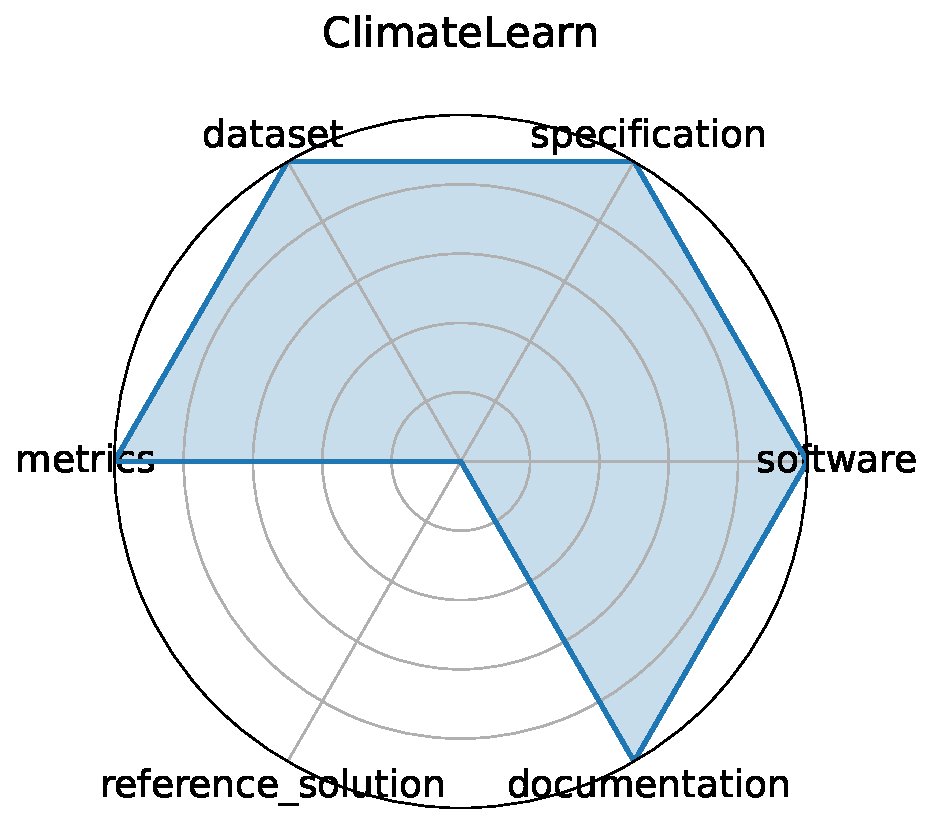
\includegraphics[width=0.2\textwidth]{climatelearn_radar.pdf}
}}
\clearpage